\documentclass[10pt,aspectratio=169]{beamer}
\usetheme{metropolis}
\usepackage{appendixnumberbeamer}
\usepackage{booktabs}
\usepackage{amsmath,amssymb}
\usepackage{graphicx}

\graphicspath{{../figures/}}
\metroset{block=fill,progressbar=frametitle}

\newcommand{\avg}[1]{\langle #1 \rangle}
\newcommand{\speaker}[1]{\hfill{\scriptsize\color{gray}#1}}

\title{How the three ensembles come to agree}
\subtitle{An exact study of a 2D quantum lattice gas}
\author{Prasang Das \and Aryan Shakya \and Dhruv Thakur}
\date{}

\begin{document}

\maketitle

\begin{frame}{The question}
  A gas can be described three ways:
  \begin{itemize}
    \item \textbf{microcanonical} --- fix energy and particle number
    \item \textbf{canonical} --- fix temperature, exchange energy with a bath
    \item \textbf{grand-canonical} --- also exchange particles
  \end{itemize}
  \vspace{0.5em}
  They agree \emph{in the thermodynamic limit}. Any finite system --- a trap, a
  simulation --- is not there yet.
  \vspace{0.5em}
  \begin{alertblock}{What we measure}
    How the agreement sets in as the lattice grows, and how interactions change it.
  \end{alertblock}
  \speaker{Prasang}
\end{frame}

\section{Model and method \hfill\normalfont\scriptsize Prasang}

\begin{frame}{The model: hard-core Bose--Hubbard}
  \[
  \hat H=-t\!\sum_{\langle i,j\rangle}\!\big(\hat b_i^\dagger \hat b_j+\text{h.c.}\big)
  +V\!\sum_{\langle i,j\rangle}\!\hat n_i \hat n_j
  \]
  \begin{columns}[T]
    \begin{column}{0.55\textwidth}
      \begin{itemize}
        \item bosons hop between neighbors ($t$)
        \item repel or attract neighbors ($V$)
        \item at most one boson per site
      \end{itemize}
    \end{column}
    \begin{column}{0.45\textwidth}
      \begin{itemize}
        \item cold atoms in an optical lattice
        \item energy in units of $t$; $k_B=1$
      \end{itemize}
    \end{column}
  \end{columns}
  \vspace{0.4em}
  {\footnotesize Not the quantum lattice-gas \emph{automaton} --- same name, different thing.}
  \speaker{Prasang}
\end{frame}

\begin{frame}{Exact diagonalization}
  \begin{itemize}
    \item $\hat H$ conserves $N$: block diagonal, one block per sector
    \item diagonalize each block \emph{fully} --- the partition sums need every level
    \item sizes $L=2,3,4$ ($M=4,9,16$ sites); half-filled block is the cost ceiling
  \end{itemize}
  \vspace{0.5em}
  One spectrum $\{E_{N,\alpha}\}$, built once and cached, feeds all three ensembles.
  \speaker{Prasang}
\end{frame}

\section{Ensembles and what to measure \hfill\normalfont\scriptsize Aryan}

\begin{frame}{Three ensembles, one spectrum}
  \begin{columns}[T]
    \begin{column}{0.33\textwidth}
      \textbf{Microcanonical}
      \[ \Omega(E,N;\Delta E) \]
      \[ S=\ln\Omega \]
    \end{column}
    \begin{column}{0.33\textwidth}
      \textbf{Canonical}
      \[ Z_N=\sum_\alpha e^{-\beta E_{N,\alpha}} \]
      \[ C_V=\beta^2\mathrm{Var}(E) \]
    \end{column}
    \begin{column}{0.33\textwidth}
      \textbf{Grand}
      \[ \Xi=\sum_N e^{\beta\mu N}Z_N \]
      \[ \partial_\mu\avg N=\beta\,\mathrm{Var}(N) \]
    \end{column}
  \end{columns}
  \vspace{0.6em}
  Each is a different weighting of the same levels.
  \speaker{Aryan}
\end{frame}

\begin{frame}{Equivalence is a fluctuation}
  Canonical weight is a Laplace transform of the count:
  \[ Z_N=\int dE\, e^{\,S(E)-\beta E}. \]
  The saddle at $S'(E^\ast)=\beta$ ties the two temperatures together; its width gives
  \[ \frac{\sigma_E}{|\avg E|}\sim\frac{1}{\sqrt M},
     \qquad \frac{\sigma_N}{\avg N}\sim\frac{1}{\sqrt M}. \]
  These ratios are the small parameters of equivalence --- and smooth spectral sums,
  so they survive on a tiny spectrum.
  \speaker{Aryan}
\end{frame}

\begin{frame}{Why not read $T$ off the entropy?}
  \begin{columns}[T]
    \begin{column}{0.52\textwidth}
      $1/T=\partial S/\partial E$ is the honest definition --- and useless here.
      \begin{itemize}
        \item $S=\ln\Omega$ is a jagged histogram
        \item slope diverges in gaps
        \item flips sign past the band center (negative $T$)
      \end{itemize}
      So we track the fluctuations instead.
    \end{column}
    \begin{column}{0.48\textwidth}
      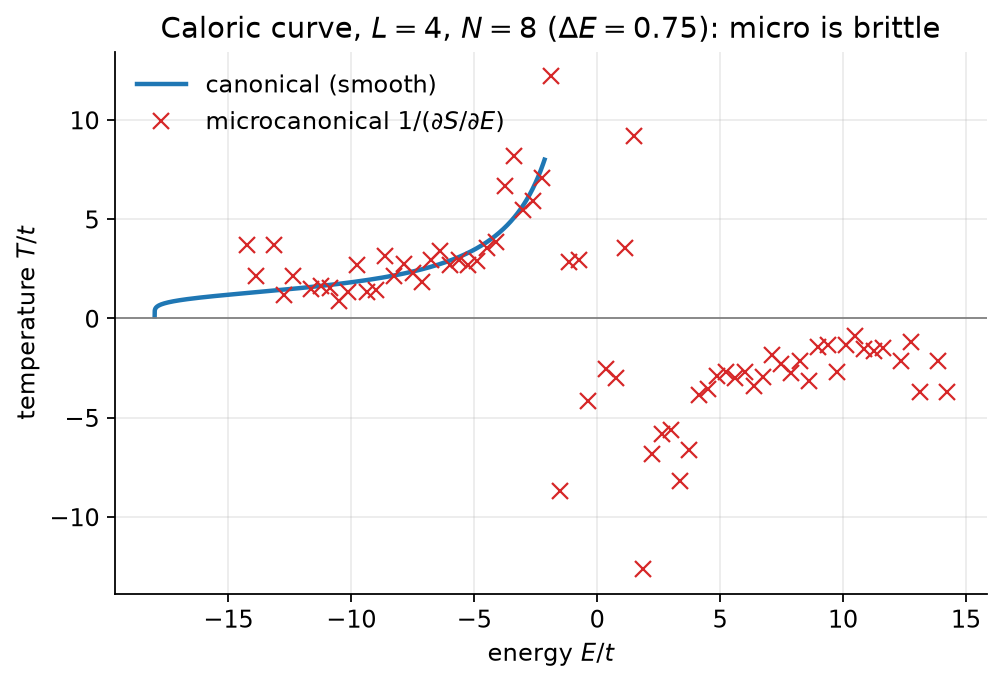
\includegraphics[width=\linewidth]{fig11_caloric_curve.png}
    \end{column}
  \end{columns}
  \speaker{Aryan}
\end{frame}

\begin{frame}{Does it compute the right thing?}
  Checked against independent references:
  \begin{itemize}
    \item one-particle band matches $-2t[\cos k_x+\cos k_y]$ to $10^{-15}$
    \item ground states match a sparse Lanczos solver
    \item $C_V=\beta^2\mathrm{Var}(E)$, $\partial_\mu\avg N=\beta\mathrm{Var}(N)$ vs numerical derivatives ($10^{-5}$)
    \item $T\to0,\infty$ limits of $S$ and $C_V$
  \end{itemize}
  \speaker{Aryan}
\end{frame}

\section{Results \hfill\normalfont\scriptsize Dhruv}

\begin{frame}{Thermodynamics behaves}
  \begin{columns}[T]
    \begin{column}{0.5\textwidth}
      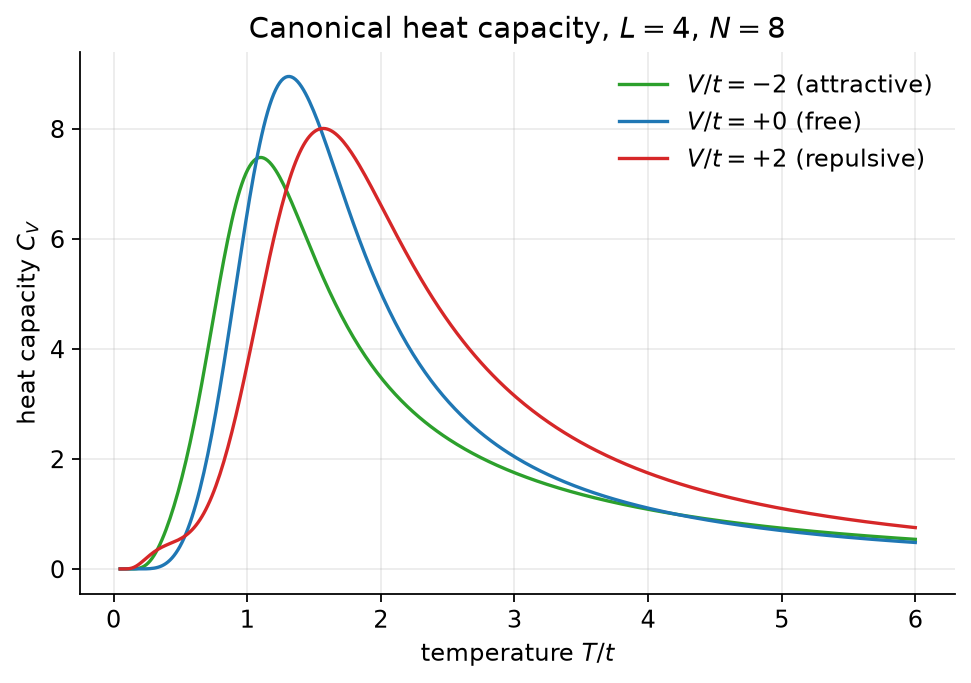
\includegraphics[width=\linewidth]{fig2_heat_capacity.png}
    \end{column}
    \begin{column}{0.5\textwidth}
      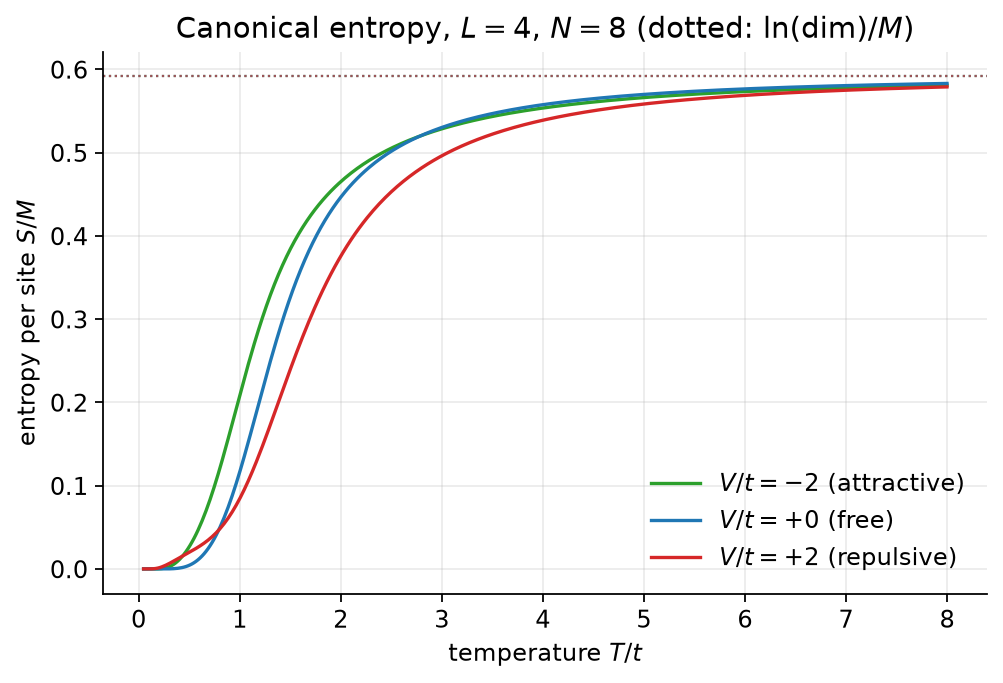
\includegraphics[width=\linewidth]{fig8_entropy_temperature.png}
    \end{column}
  \end{columns}
  Schottky-like heat capacity; entropy climbs from $0$ to $\ln(\dim)/M$. Interaction
  shifts the scale, not the shape.
  \speaker{Dhruv}
\end{frame}

\begin{frame}{Equivalence emerges with size}
  \begin{center}
    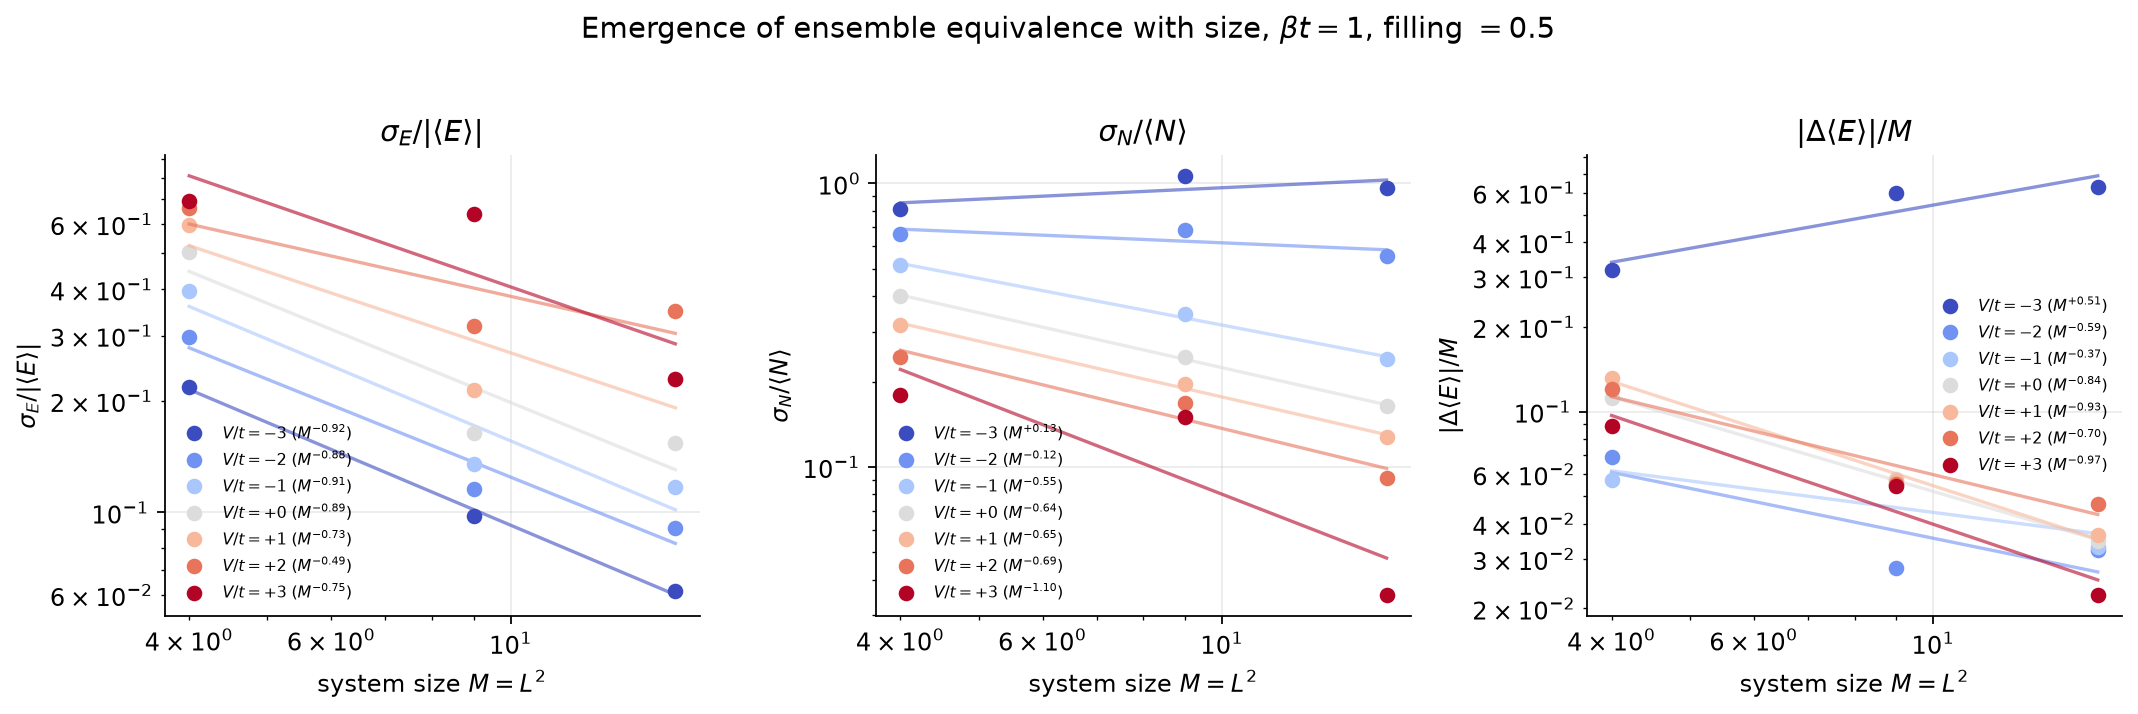
\includegraphics[width=0.96\linewidth]{fig6_scaling.png}
  \end{center}
  Free and repulsive: all three discrepancies fall with $M$, near $M^{-1/2}$.
  \speaker{Dhruv}
\end{frame}

\begin{frame}{Attraction breaks it --- in the number channel}
  \begin{columns}[T]
    \begin{column}{0.5\textwidth}
      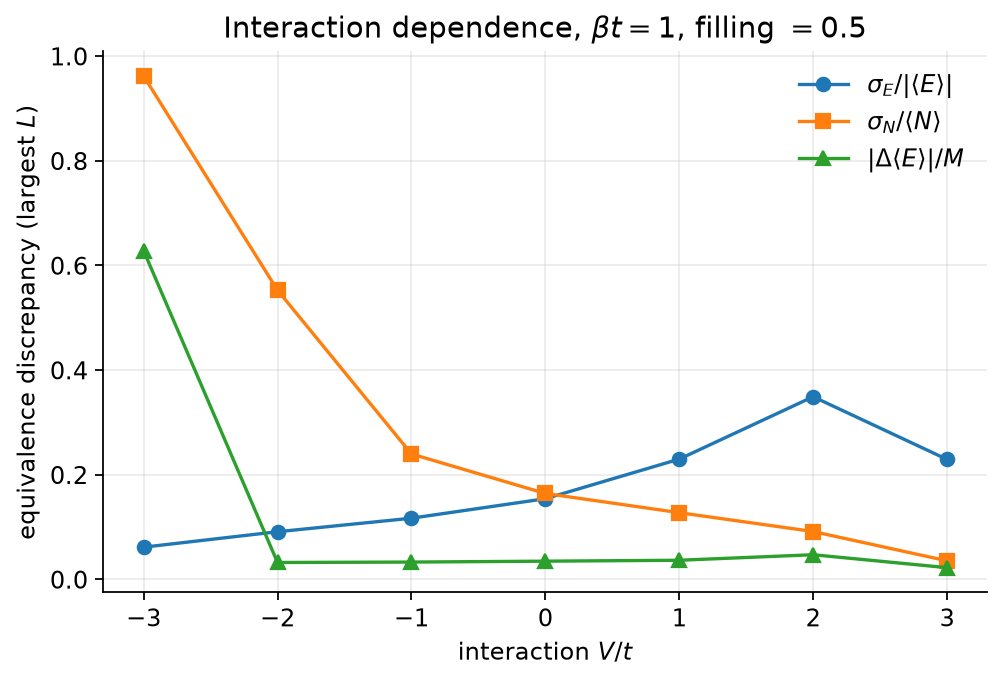
\includegraphics[width=\linewidth]{fig7_interaction.png}
    \end{column}
    \begin{column}{0.5\textwidth}
      \small
      \begin{tabular}{rr r}
        \toprule
        $V/t$ & $p(\sigma_N/\avg N)$ & $\sigma_N/\avg N$\\
        \midrule
        $-3$ & $+0.13$ & 0.96\\
        $0$  & $-0.64$ & 0.16\\
        $+3$ & $-1.10$ & 0.04\\
        \bottomrule
      \end{tabular}
      \vspace{0.6em}

      At $V/t=-3$ the exponent is \textbf{positive}: the mismatch \emph{grows} with
      size --- the gas wants to phase separate.
    \end{column}
  \end{columns}
  \speaker{Dhruv}
\end{frame}

\begin{frame}[standout]{Takeaway}
  The ensembles converge for free and repulsive particles,
  and \emph{diverge} for attractive ones --- in the particle number, where
  phase separation lives.

  \vspace{0.5em}
  Measured through fluctuations, because the microcanonical thermometer fails on
  small bounded spectra.
\end{frame}

\appendix
\begin{frame}[standout]{Thank you}
  \centering
  Prasang Das \quad Aryan Shakya \quad Dhruv Thakur\\[0.5em]
  {\footnotesize Hard-core Bose--Hubbard model, exact diagonalization}
\end{frame}

\end{document}
